\section{Radix-sort}
\subsection{Instruction}
Show the steps that a radix sort takes when sorting the following array of integer keys:
\begin{center}
\textbf{832 91 411 172 243 573 326 292 682 489 96}
\end{center}

\subsection{Run Radix-Sort through the array}
\textbf{The original array}
\\
\\
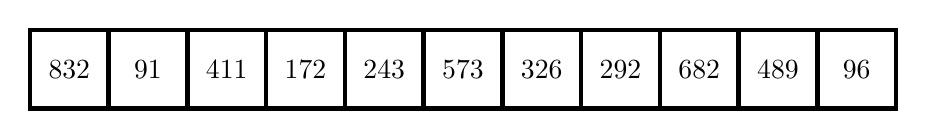
\begin{tikzpicture}
        [box/.style={rectangle,draw=black, ultra thick, minimum size=1cm},]
\foreach \x/\y in {0/832, 1/91, 2/411, 3/172, 4/243, 5/573, 6/326, 7/292, 8/682, 9/489, 10/96}
        \node[box] at (\x,0){\y};
\end{tikzpicture}
\\
\\
\textbf{Run the first round of radix-sort with the most right bit of each key}
\\
\\
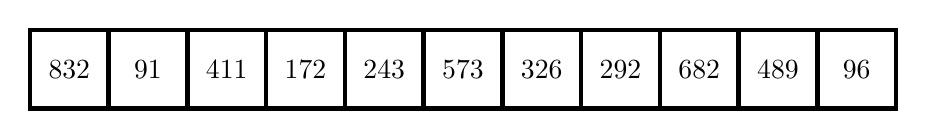
\begin{tikzpicture}
        [box/.style={rectangle,draw=black, ultra thick, minimum size=1cm},]
\foreach \x/\y in {0/83\ul{2}, 1/9\ul{1}, 2/41\ul{1}, 3/17\ul{2}, 4/24\ul{3}, 5/57\ul{3}, 6/32\ul{6}, 7/29\ul{2}, 8/68\ul{2}, 9/48\ul{9}, 10/9\ul{6}}
        \node[box] at (\x,0){\y};
\end{tikzpicture}
\\
\\
\textbf{Result as: }
\\
\\
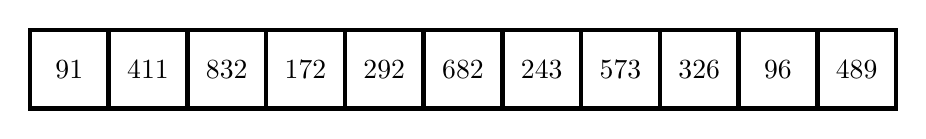
\begin{tikzpicture}
        [box/.style={rectangle,draw=black, ultra thick, minimum size=1cm},]
\foreach \x/\y in {0/91, 1/411, 2/832, 3/172, 4/292, 5/682, 6/243, 7/573, 8/326, 9/96, 10/489}
        \node[box] at (\x,0){\y};
\end{tikzpicture}
\\
\\
\textbf{Run the second round with the second bit}
\\
\\
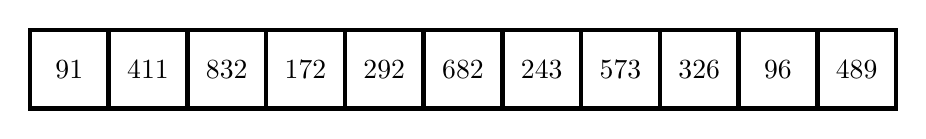
\begin{tikzpicture}
        [box/.style={rectangle,draw=black, ultra thick, minimum size=1cm},]
\foreach \x/\y in {0/\ul{9}1, 1/4\ul{1}1, 2/8\ul{3}2, 3/1\ul{7}2, 4/2\ul{9}2, 5/6\ul{8}2, 6/2\ul{4}3, 7/5\ul{7}3, 8/3\ul{2}6, 9/\ul{9}6, 10/4\ul{8}9}
        \node[box] at (\x,0){\y};
\end{tikzpicture}
\\
\\
\textbf{Result as: }
\\
\\
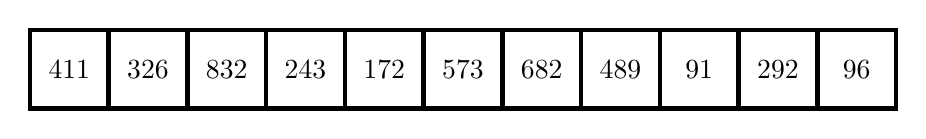
\begin{tikzpicture}
        [box/.style={rectangle,draw=black, ultra thick, minimum size=1cm},]
\foreach \x/\y in {0/411, 1/326, 2/832, 3/243, 4/172, 5/573, 6/682, 7/489, 8/91, 9/292, 10/96}
        \node[box] at (\x,0){\y};
\end{tikzpicture}
\\
\\
\textbf{Run the third round with the third bit}
\\
\\
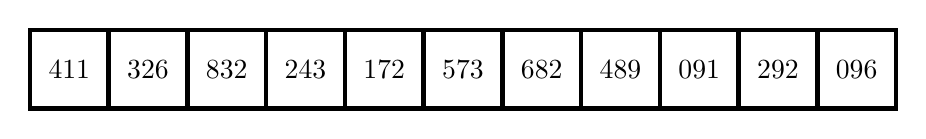
\begin{tikzpicture}
        [box/.style={rectangle,draw=black, ultra thick, minimum size=1cm},]
\foreach \x/\y in {0/\ul{4}11, 1/\ul{3}26, 2/\ul{8}32, 3/\ul{2}43, 4/\ul{1}72, 5/\ul{5}73, 6/\ul{6}82, 7/\ul{4}89, 8/\ul{0}91, 9/\ul{2}92, 10/\ul{0}96}
        \node[box] at (\x,0){\y};
\end{tikzpicture}
\\
\\
\textbf{Result as: }
\\
\\
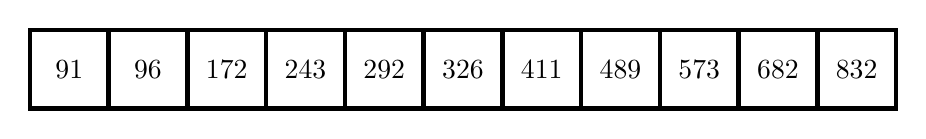
\begin{tikzpicture}
        [box/.style={rectangle,draw=black, ultra thick, minimum size=1cm},]
\foreach \x/\y in {0/91, 1/96, 2/172, 3/243, 4/292, 5/326, 6/411, 7/489, 8/573, 9/682, 10/832}
        \node[box] at (\x,0){\y};
\end{tikzpicture}
\\
\\
\textbf{The maximum length of a key is 3. The algorithm has gone through 3 rounds $\rightarrow$ Terminate radix-sort. The array  of integer keys was sorted.}